%% The following is a directive for TeXShop to indicate the main file
%%!TEX root = ../diss.tex

% Some of this content is from the 2018 HPG paper with JB as first author. Rest of this chapter is new from AARTS1
%% paper title: Heterogeneous distribution of trastuzumab in HER2-positive xenografts and metastases: role of the tumour microenvironment

\chapter{Applications of HPG in evaluating antiangiogenic agents}
\label{ch:HPG2}

\section{Background}

Treatment options for patients with the aggressive HER2-positive form of breast cancer continue to improve, though metastatic breast cancer remains a largely incurable disease.
Brain metastases are of particular importance in HER2-positive breast cancer patients, as with improved treatments and prolonged survival the incidence of brain metastases as the first evidence of relapse has increased [1, 2].
This effect has been attributed to the phenomenon of the blood-brain barrier (BBB) creating a sanctuary site by preventing drug access [3, 4].
Antibody-based therapeutics such as trastuzumab are proposed to have difficulty crossing the BBB and therefore brain metastases evade drug activity [1, 5, 6].
In addition to the BBB, specific characteristics of the tumour microenvironment, beginning with a relative paucity of functional vessels, can thwart the access of drugs to their targets such that a population of under-exposed cells may survive and repopulate the tumour [7].
We have demonstrated that many small molecule cytotoxics have limited tumour tissue penetration in both in vivo and in vivo model systems due to difficulties with drug supply, flux through tissue, consumption or sequestration by cancer cells close to blood vessels [8, 9, 10, 11, 12].

Macromolecular compounds such as \ac{MAb} face particular extravascular distribution difficulties due to their high molecular weights and target-binding affinity [13, 14].
The relatively slow distribution of MAbs has been attributed to the binding site barrier hypothesis (BSBH), where in the case of high affinity binding of the MAb to antigen, MAb distribution is limited by its binding in the presence of ample antigen [15].
Data from our lab in the vector overexpressed MDA-435-LCC6HER2 model showed that despite the ability of trastuzumab to distribute far from vessels in tumours with relatively even HER2 distribution, there persisted HER2-positive tissue with poor access to trastuzumab after peak plasma exposures [16].
Heterogeneity is very striking at the vessel level, as trastuzumab is able to extravasate from only a subpopulation of perfused vessels.
Other groups have also demonstrated a limitation on the accumulation of trastuzumab in tumours, focusing on net tumour accumulation [13, 14, 17].

The ability of a drug to access and affect all its target cells is intuitively crucial for treatment success.
The relatively slow distribution of MAbs through the interstitium in solid tumours is recognized, but the long half-life of MAbs and prolonged plasma exposure is expected to ensure adequate time to access all the tissues in most treatment scenarios.
However, we have found that in addition to distributing slowly, MAbs experience additional barriers, leaving some areas of tissue with inadequate drug exposure.
The aim for this study was to use HER2-positive tumour and metastases models of cancer to determine potential limits to trastuzumab access that may represent a mechanism of resistance to targete d therapies.
The microenvironments of HER2-positive tumours and metastases are examined in detail using immunohistochemistry maps, 3D tissue models and dynamic imaging of tumour vasculature.

\section{Methods}

\subsection{Reagents}

Trastuzumab and bevacizumab (Roche, Genentech) were provided by the British Columbia Cancer Agency pharmacy; dilutions to 1-2 mg/ml were prepared in sterile 0.9\% NaCl before intra-peritoneal (i.p.) injection.
Human isotype control IgG1 (Sigma) was administered from similar concentrations.
Trastuzumab and IgG antibodies for use in combination with bevacizumab were tagged with fluorescent labels according to Alexa Fluor 546 Protein Labeling Kit (ThermoFisher) instructions.
Hypoxia marker pimonidazole (Hypoxyprobe) was administered at 60 mg/kg as an i.p.
injection 2 h prior to tissue harvest.
Fluorescent dye DiOC7(3) (Molecular Probes), 0.6 mg/ml dissolved in 75\% (v/v) dimethyl sulfoxide/25\% sterile H2O, was administered intravenously as a marker of vessel perfusion 5 min prior to tissue harvest [18].

\subsection{Mice and tumours}

Female NOD-SCID mice weighing 20-28 g between 8 and 16 weeks of age were bred and maintained in our institutional pathogen free animal facility.
Mice were implanted with 60 day 17-$\beta$-estradiol pellets (Innovative Research of America) subcutaneously 3 days before implantation of BT474 or MDA-MB-361 tumours.
Tumors were implanted as single cell suspensions (2-10�10$^6$ cells) into the subcutaneous sacral region or into the inguinal mammary fat pads.
Metastases models were implanted as single cell suspensions (2-5�10$^5$ cells per implant) as i.v. or i.p. injections for SKOV3 or BT474 models, or as intra-cardiac (i.c.) injection for MDA-MDA-MB-231-BR-HER2 models, with animals euthanized a maximum of 23 days after implant.

\subsection{MRI}
MRI experiments were performed at the UBC MRI Research Centre on a 7T Bruker Biospec 70/30 scanner at room temperature with a combination volume (transmit)/surface (receive) coil.
DCE-MR imaging data was collected as previously described [19].
Gadovist (Bayer Healthcare) was administered by i.v. catheter as a 5 $\mu$L/g bolus dose from 60 mM solution.
Macromolecular contrast agent hyperbranched polyglycerol (HPG-GdF, 500 kDa) was synthesized as previously described [20, 21] and administered as a 6 $\mu$L/g bolus dose from 100 mg/mL (0.2 mM).
Regions of interest (ROI) were drawn on T2-weighted RARE images to outline the tumour using ImageJ (NIH) and all other MR analysis was performed using Python.
Area Under the Curves (AUC) for Gadovist was determined from the common injection time point to 60 s.
A two-parameter linear model was applied to characterize \ac{HPG-GdF} signal-intensity curves for fractional plasma volume (fPV) determined by the rapid increase at time of injection and for apparent permeability surface area product (aPS) calculated as the slope of later enhancement, as previously described [19].
Both MR and histological modalities imaged slices in the plane perpendicular to an implanted fiducial marker tube to minimize angular differences between MR and histological image slices [22].

\subsection{Immunohistochemistry}
The general immunohistochemical procedure used has been previously reported [16].
Briefly, 10 $\mu$m tumour cryosections were air-dried, imaged for native DiOC7(3) or Alexa 546-tagged trastuzumab fluorescence, and fixed in 50\% (v/v) acetone/methanol for 10 min at room temperature.
Trastuzumab and IgG were visualized in sections using Alexa 546 goat anti-human secondary antibody (Invitrogen).
HER2 was subsequently stained with 2.2�10$^{-3}$ mg/mL trastuzumab as a primary detection antibody and goat anti-human Alexa 546 secondary.
Additional staining was performed using antibodies to PECAM/CD31 (BD PharMingen), pimonidazole (hypoxprobe) collagen IV (Gene Tex) and $\alpha$SMA (Abcam).
Visualization of primary detection antibodies was done using Alexa fluorescence secondary antibodies of appropriate species using 488 nm, 647 nm and 750 nm wavelengths.
Nuclear density was stained using Hoechst 33342 (Thermofisher) and imaged at 380 nm.

\subsection{Image acquisition and analysis}
Sections were imaged as previously described [9] using a system of tiling adjacent microscope fields of view at a resolution of 0.75 $\mu$m/pixel.
Using ImageJ [23] and user-supplied algorithms, images were superimposed and manually cropped to tumour tissue boundaries with staining artifacts and necrosis removed.
False color images were constructed in ImageJ by converting greyscale images to color and overlaying selected layers: trastuzumab (magenta), HER2 (blue or grey), Hoechst 33342 (grey), CD31 (blue), carbocyanine (cyan), pimonidazole (green) and $\alpha$SMA or CIV (red).
Positive fluorescent staining is reported as average intensity (range 1-255) for pimonidazole, trastuzumab and HER2.
Perfused vascular density was determined by applying a threshold to CD31 and DiOC7(3) images, with neighboring positive pixels grouped as ``objects''; CD31 objects with a minimum 20\% overlap with DiOC7(3) objects were determined to be perfused vessels.
All image pixels were sorted based on their nearest perfused vessel and the average distance is reported as a repeatable measure of vascular density.

\section{Results}

\subsection{Measures of vascular density, architecture and function do not consistently correlate with heterogeneous patterns of trastuzumab distribution}

Significant inter-vessel heterogeneity in trastuzumab distribution is seen in orthotopic BT474 xenografts, with neighboring patent vessels often showing variable amounts of trastuzumab bound to perivascular cells (Fig.
4a), similar to previous findings in MDA-435-LCC6 vector-overexpressing HER2-positive tumours [16].
Non-patent vessels (red arrows) never have extravascular trastuzumab, suggesting intermittent perfusion is not a significant mechanism for reduced trastuzumab access.
The same inter-vessel heterogeneity is seen in MDA-MB-361 tumours where vascular function dynamics were further characterized by imaging MR contrast agent Gadovist accumulation (Fig.
4b).
Matched histology slices were stained for the location of trastuzumab, vascular patency and markers of vascular maturity CIV and $\alpha$SMA.
Some regions are high for MR-imaged Gadovist uptake, reflecting high vascular function, but these do not consistently co-register with regions of high trastuzumab distribution in histology sections.
A quantitative correlation between Gadovist AUC and trastuzumab in matched image slices obtained from multiple tumours was not evident.
Similarly, neither $\alpha$SMA nor CIV are present to a greater degree proximal to vessels with or without trastuzumab bound to perivascular cells.

\begin{figure}[htbp] %  figure placement: here, top, bottom, or page
   \centering
   \includegraphics[width=0.8\textwidth]{hpg/hpg-paper2-images/Fig4.pdf} 
   \captionsetup{width=1.2\linewidth}
   \caption{Distribution of Tz in vivo relative to tumour blood vessels. 
   A) Magnified region of a BT474 xenograft grown orthotopically in inguinal mammary fat pad and treated with 10 mg/kg trastuzumab for 24 h. 
   Trastuzumab extravasates from vessels heterogeneously, with many patent vessels showing no extravascular bound trastuzumab (green arrows) even when adjacent to other patent vessels that do have perivascular trastuzumab. 
   Carbocyanine fluorescent dye (cyan) around CD31 stained vessels (blue) indicates patency; non-patent vessels are indicated (red arrows). 
   B) DCE-MR imaging of Gadovist accumulation (GadovistAUC60) in MDA-MB-361 tumours is compared with detailed histology mapping of matched histological sections. 
   Regions with greatest AUC60(Gadovist), reflecting greatest vascular function, do not consistently correspond to areas of greater trastuzumab distribution (red arrow); this is also demonstrated quantitatively where matched slices were plotted for amount of bound trastuzumab and AUC60(Gadovist). 
   The same sections were stained for vascular architectural markers $\alpha$SMA and CIV (both shown in red), neither of which exhibit a pattern of distribution similar to the presence or absence of trastuzumab (whole sections top; zoomed in region below).}
   \label{hpgpaper2:fig4}
\end{figure}

\subsection{Dynamic vascular permeability and blood volume measurements do not consistently relate to patterns of trastuzumab distribution}

The histological measure of perfusion using carbocyanine is a useful indication of vessel patency, however it is static and therefore its interpretation is limited.
The role of vascular function on trastuzumab distribution was further investigated using dynamic contrast enhanced MRI (DCE-MRI) of a high molecular weight contrast agent, \ac{HPG-GdF} (MW 500 kDa) (Fig.
6).
As previously described, repeat imaging of contrast agent presence in the tumours is analysed and the initial appearance of \ac{HPG-GdF} reflects \ac{fPV} and its accumulation over time indicates the apparent permeability surface area (aPS) [19].
Tumors were excised immediately after imaging; corresponding histological sections are compared to the DCE-MRI derived parameter maps.
BT474 tumours have microregionally variable levels of both \ac{fPV} and \ac{aPS}, each exhibiting regions of distinction.
Regions of high \ac{fPV} are well matched by histological images of carbocyanine that indicate areas of very high perfusion but some of these regions do not have any significant accumulation of trastuzumab.
The reverse can also be found, where regions with relatively low \ac{fPV} correspond to high trastuzumab.
Similarly, there are some significant trastuzumab accumulation areas that have relatively low \ac{aPS} while some high \ac{aPS} values correspond to areas with relatively low trastuzumab.
Examples of good or bad correlation between vascular function and trastuzumab distribution are highlighted with arrows and suggest that neither of the MRI-derived parameters consistently or adequately explain microregional distribution of trastuzumab.

\begin{figure}[htbp] %  figure placement: here, top, bottom, or page
   \centering
   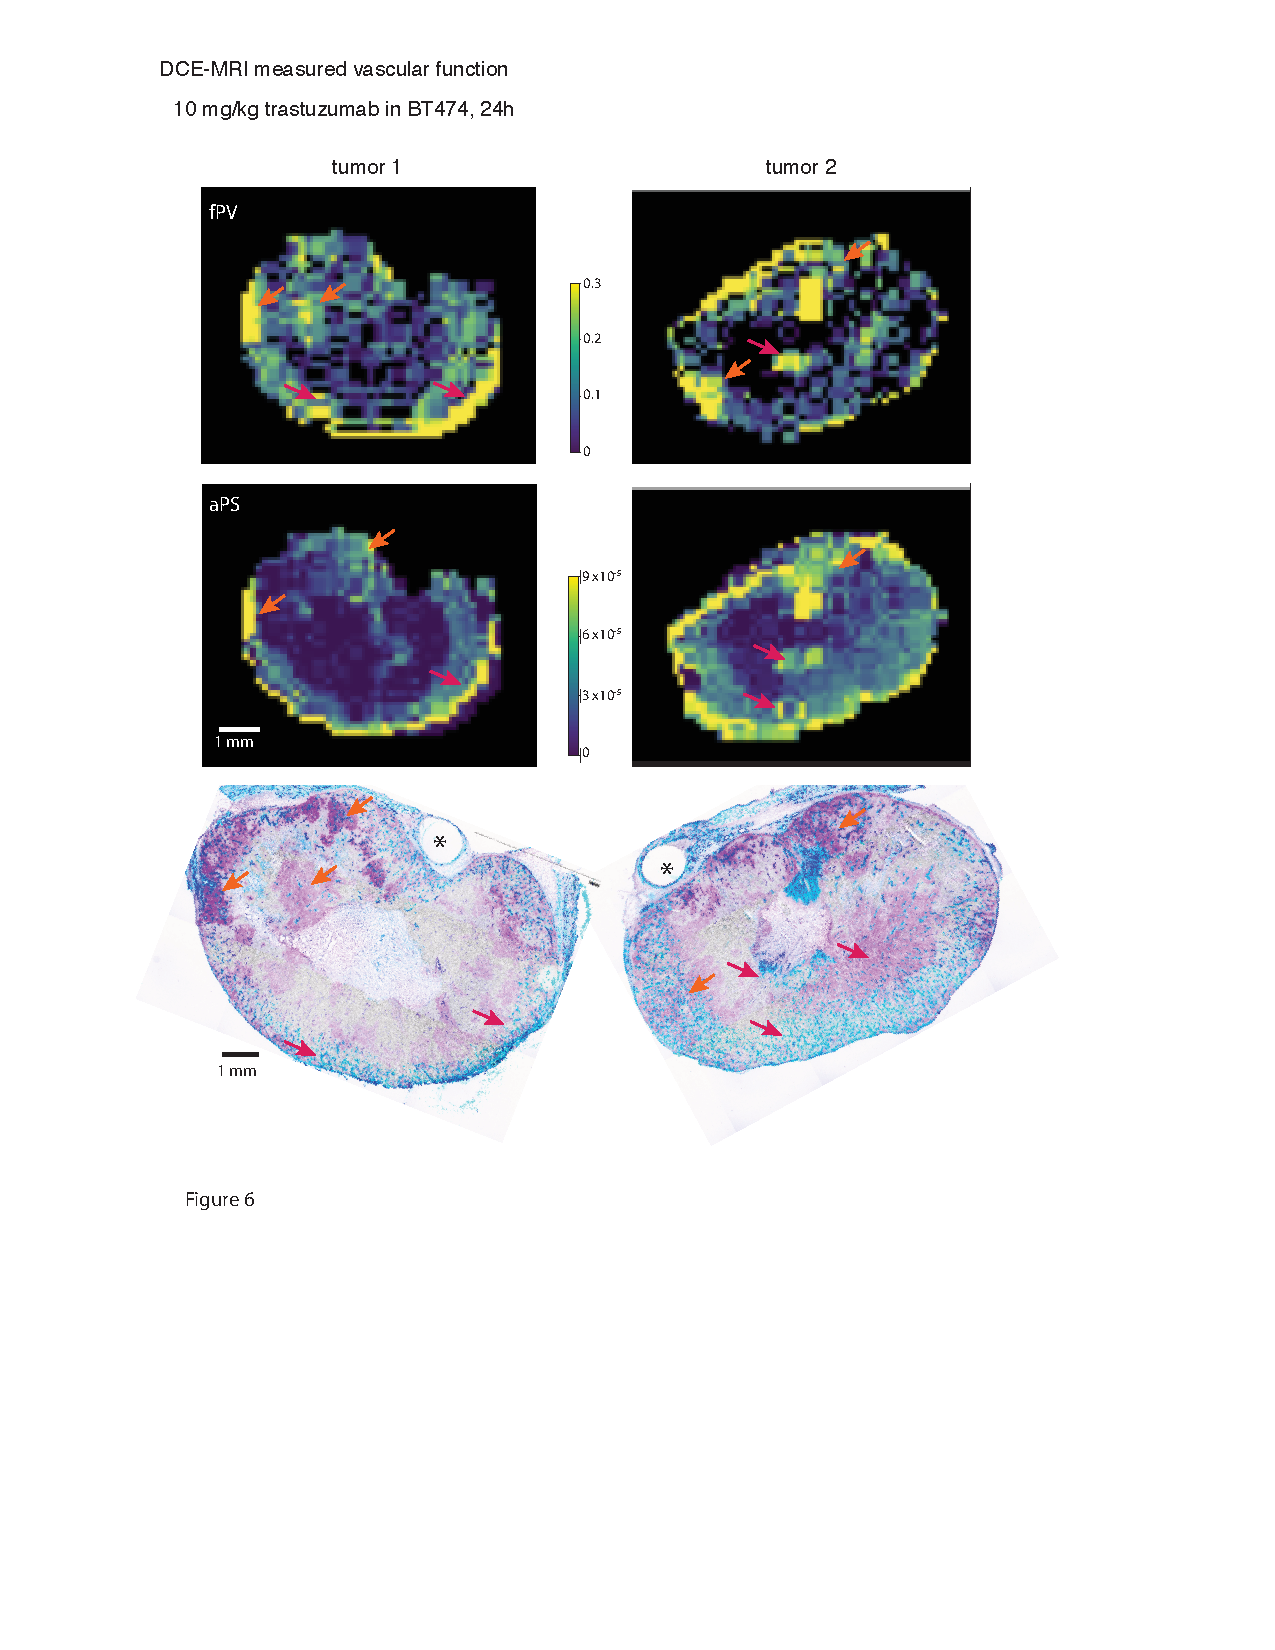
\includegraphics[width=\textwidth]{hpg/hpg-paper2-images/Fig6.pdf} 
   \caption{Dynamic measurements of vascular function relative to trastuzumab distribution. BT474 tumours were imaged at a 7T MRI scanner and uptake of \ac{HPG-GdF} contrast agent (500 kDa) was measured. 
   Parameter maps show calculated values for fractional plasma volume (fPV) and apparent permeability surface area (aPS), reflecting vascular perfusion and permeability respectively. 
   Matched histology sections are stained for bound trastuzumab (magenta) administered at 10 mg/kg 24 h prior to imaging and tissue collection, and for HER2 (grey), carbocyanine marker of perfusion (cyan) and for CD31 vasculature (blue). 
   Areas of vascular function (MRI) and trastuzumab (histology) correlation are indicated (orange arrows) in both modalities; example areas of poor matching are also shown (red arrows). 
   Stars indicate location of fiducial markers for multi-modal slice comparison.}
   \label{hpgpaper2:fig6}
\end{figure}

\section{Discussion}

This study has shown direct evidence of poor trastuzumab access to metastases of the brain in a preclinical model.
Small clusters of cells that are immediately surrounded by highly perfused brain, liver or lung tissues may remain incompletely or in some cases totally unbound for trastuzumab.
Some avascular metastases of the brain may be outside the BBB and therefore have poor access to trastuzumab, while larger lesions with active angiogenesis and blood vessel support may have a blood-tumour barrier (BTB) with greater trastuzumab delivery, however we have shown that microregional distribution of trastuzumab can remain highly heterogeneous and incomplete even when delivered by vessels within HER2-positive lesions.
Our data are in agreement with other studies evaluating the permeability of brain metastases, which have found no correlation between metastases size, vessel density, aggressiveness or morphology and their permeability [5, 24].
Mittapalli et al. have used mathematical modeling and MRI data to show a limit in the vascular pore size of MDA-MB-231-BR-HER2 metastases that would preclude access to MAbs including trastuzumab [25].
Other groups have also shown poor trastuzumab access in this model [26, 27].
As found here, trastuzumab has been detected in larger brain lesions in murine models [28] where higher systemic doses of the MAb were required to achieve anti-cancer efficacy seen for tumours grown in the mammary fat pad.
Accumulation over time has also been noted in patient metastases including those of the brain, where labeled antibodies were used for diagnostic purposes using PET [29, 30].
It is unknown if human tumours or metastases exhibit the same barriers to MAb access.
As we have shown, access of trastuzumab to metastases and the distribution within can be highly heterogeneous, and is likely to be highly model and patient specific.
Ultimately, a majority of patients treated with trastuzumab eventually experience progression and relapse.
The rate of brain metastases has increased for HER2-positive patients following treatment with trastuzumab, suggesting the MAb therapeutic is less effective for tumours `behind' the BBB than in metastases elsewhere such as the liver and lung [6].
Here we show direct evidence of poor trastuzumab access to HER2-positive brain metastases and suggest that this confirms non-uniform access of MAbs to cancers and metastases may be driving a significant portion of resistance to their effects.

Using tumour mapping analysis and DCE-MRI we further examined the impacts of HER2 expression, tumour blood vessel architecture, vascular function and the tumour microenvironment on the patterns of distribution of trastuzumab in primary and metastatic models.
We have observed that even when trastuzumab does have access to tumour tissues, the pattern of distribution is highly heterogeneous, similar to our previous work in a vector-overexpressing HER2-positive breast cancer model [16].
Other groups demonstrating a limitation on the accumulation of trastuzumab in preclinical tumours have focused on net tumour accumulation and suggest that a major limitation to MAb distribution is their difficulty distributing through the solid tumour tissue in the extravascular space [13, 14, 17].
In humans MAbs have a long half-life and are administered for many months.
The pharmacokinetic parameters of MAbs are therefore thought to likely accommodate relatively slow distribution of MAbs through the interstitium [14, 31].
However, our 3D tissue disc data shows trastuzumab is able to diffuse relatively well through tumour tissues in vivo in conditions of poor convective flow similar to an environment with high interstitial fluid pressure in vivo.
Neither is trastuzumab distribution limited by tight binding to antigen proximal to vessels as suggested by the binding-site barrier hypothesis [15], as it reaches distances > 150 $\mu$m from sources within 24 h despite high HER2 expression.
This distance is similar to the diffusion limit for oxygen, therefore most tumour tissues are within this 150 $\mu$m range of a blood vessel and could be expected to have adequate exposure.
These data suggest that neither the BSBH nor high interstitial fluid pressure adequately explain microregional variation in trastuzumab binding.
Given the incomplete access of trastuzumab seen in our models, other vessel- and tissue-level barriers appear to limit its distribution in the tumour microenvironment.

One barrier to MAb distribution appears to be the presence of tight junctions, labeled using ZO-1.
However, these continuous barriers are not seen in vivo where inter-vessel heterogeneity occurs and even neighboring perfused vessels exhibit dramatic differences in the amount of bound drug on their perivascular cells.
Vascular maturity and architecture has also been attributed to poor drug access [32], however, no correlation between markers for aSMA or CIV and the relative distribution of trastuzumab has been found.Higher doses and longer exposures do lead to higher numbers of vessels with perivascular trastuzumab, suggesting that some degree of intermittent perfusion or very poorly permeable vessels impact the observed microregional heterogeneity.
Non-perfused vessels have not been observed to have trastuzumab on perivascular cells, which suggests intermittent perfusion is an unlikely mechanism for observed inter-vessel heterogeneity.
Dynamic measurements of perfusion and permeability derived from DCE-MR imaging of high molecular weight contrast agent \ac{HPG-GdF} (500 kDa) suggest the intuitive relationship between vascular function and drug access is important, but does not consistently explain the heterogeneous patterns of drug distribution seen.
Areas of highly perfused tissue marked by carbocyanine in histological sections correspond to areas of high perfusion and/or permeability in MRI.
However, these tumour areas of high vascular function described in both imaging modalities may or may not have bound trastuzumab.
Similarly, regions with substantial amounts of bound trastuzumab do not necessarily correspond to areas of high perfusion or permeability measured using \ac{aPS} and \ac{fPV}.
HPG-GdF-derived parameters \ac{fPV} and \ac{aPS} arise under conditions that are closer to a permeability-limited regime than standard low-molecular weight contrast agents.
However, in the highly chaotic vascular environment of tumours we can still expect these MR-derived parameters of vascular function to not be completely independent of each other.

All in vivo models investigated were found to be sensitive to the effects of bevacizumab, a monoclonal antibody that binds VEGF-A and decreases vascular permeability [33].
In our xenograft studies we see a dramatic reduction in the accumulation of trastuzumab in tumours when following pre-treatment with bevacizumab.
The majority of tumour blood vessels cease to have extravasated trastuzumab bound to perivascular cells.
These detailed images of the microenvironment highlighting reduced distribution at the vessel level agree with previous studies showing average reductions in trastuzumab delivery to the whole tumour [34, 35].
In some cases VEGF ablation changes tumour vasculature, either the density or the fraction of perfused or mature vessels and the resulting overall function of tumour vasculature, but did not do so measurably in these tumours where neither the proportion of perfused vessels nor the amount of tumour hypoxia changed.

The clinical impact of combination treatments is unclear, largely due to the difficulty in measuring drug distribution directly.
Addition of bevacizumab did not improve outcomes for metastatic breast cancer patients being treated with docetaxel and trastuzumab [36].
Overall, poor clinical results have been found when combining VEGF ablation therapies with trastuzumab (reviewed in [37]).
The potential risks of combining MAbs and anti-angiogenic treatments have been recognized, and many publications and reviews in the pre-clinical and clinical fields of have called for investigations regarding optimal treatment and scheduling regimens for these combinations [37, 38, 39, 40, 41, 42, 43].

New strategies that are able to more effectively target and kill cancer cells, particularly metastatic disease, are urgently required.
Efforts to vary antigen-binding affinities and the size of MAb fragments have been explored to improve their distribution through the extravascular compartment [13, 14].
Our data highlight the importance of also considering access of antibodies to target tumour tissues and whether microregional distribution of MAb therapeutics may be affected when combined with vascular damaging agents or when targeting occult metastases.
Improvements to MAb anti-cancer activity could be made in selection of combination therapies and the design of treatment schedules, as well as in the design of novel targeted drugs.
Efforts to examine these phenomena in the clinic would be of significant interest.

\section{Conclusion}

We have shown evidence for poor distribution and access of the MAb trastuzumab in preclinical tumours through direct visualization of bound drug, with particular implications for metastatic tumours, including those of the brain.
Our data suggest that the tumour microenvironment and tissue- and vessel-level barriers to drug distribution could effectively limit access of the drug to all its target cells.
These effects appear to be more important than slow interstitial distribution resulting from high interstitial fluid pressures or high binding affinity to HER2.
Further, administering trastuzumab in combination with vascular disrupting agents could significantly impact its activity via reducing access.



\endinput
